\documentclass[14pt,compress]{beamer}
\usepackage[spanish]{babel}
\usepackage[utf8]{inputenc}
\usepackage{presento}

%configuration file
%\setbeamercolor{title}{fg=DarkRed}
%\setbeamercolor{frametitle}{fg=DarkRed}
\setbeamercolor{normal text}{fg=darkgray}
\usebeamercolor[fg]{normal text}
%\setbeamercolor{block title}{fg=black,bg=Fern!25!white}
%\setbeamercolor{block body}{fg=black,bg=Fern!25!white}
%\setbeamercolor{alerted text}{fg=AlertColor}
%\setbeamercolor{itemize item}{fg=Charcoal}

\usepackage[font={color=dimgray},figurename={ },labelfont={ }]{caption}



% personal data
\newcommand{\mycongress}{\setnote{\color{darkgray}\small
I Encuentro Nacional de Din\'amica Cu\'antica en la Materia}}
\newcommand{\myTitle}{\color{orange}{\fontsize{27}{29}\selectfont 
Implementación de Métodos de Aprendizaje Automatizado
en problemas colisionales}}
\newcommand{\myemail}{\setnote{\color{darkgray}\scriptsize 
alemendez@iafe.uba.ar}}
\newcommand{\myDetails}{\setnote{\color{darkgray}\small 
1 de Septiembre -- Buenos Aires}}

% colors: black, blue, brown, cyan, darkgray, gray, green, 
% lightgray, lime, magenta, olive, orange, pink, purple, red, teal, 
% violet, white, yellow.

\begin{document}
%%%%%%%%%%%%%%%%%%%%%%%%%%%%%%%%%%%%%%%%%%%%%%%%%%%%%%%%%%%%%%%%%
\begin{frame}[plain]
\vfill
\mycongress

\vspace{0.7cm}
\myTitle
% \hline

\noindent\makebox[\linewidth]{\rule{0.85\paperwidth}{0.7pt}}
\vfill

% \vspace{0.5cm}
\hspace{2.75cm}\text{\color{teal}{\normalsize Alejandra Mendez,}} \\
\hspace{2.75cm}\text{\color{teal}{\normalsize Juan Di Filippo,}} \\
\hspace{2.75cm}\text{\color{teal}{\normalsize Sebasti\'an L\'opez,}} \\
\hspace{2.75cm}\text{\color{teal}{\normalsize Dar\'io Mitnik,}} \\
\vfill
\vspace{-0.25cm}
\hspace{2.5cm}\myemail
\vfill
\begin{tikzpicture}[remember picture,overlay]
\node[xshift=-10.7cm,yshift=-6.45cm] at (current page.north east) 
{\includegraphics[width=0.28\textwidth]{iafe.jpg}};
\end{tikzpicture}

\vspace{-0.5cm}
\centering
\myDetails 

\end{frame}
%%%%%%%%%%%%%%%%%%%%%%%%%%%%%%%%%%%%%%%%%%%%%%%%%%%%%%%%%%%%%%%%%%%%%%%%
\section{Machine Learning}
%%%%%%%%%%%%%%%%%%%%%%%%%%%%%%%%%%%%%%%%%%%%%%%%%%%%%%%%%%%%%%%%%%%%%%%%
\framepic[1.]{figures/mlcover_modif.png}{
 \begin{textblock}{8}(6.5,-2.2)
    {\color{orange0}
\text{\huge \bf Machine} \\
\vspace{2pt}
\text{\huge\bf Learning}}
 \end{textblock} }
%%%%%%%%%%%%%%%%%%%%%%%%%%%%%%%%%%%%%%%%%%%%%%%%%%%%%%%%%%%%%%%%%%%%%%%%
\framepic[1.]{figures/ionization.png}{}
%%%%%%%%%%%%%%%%%%%%%%%%%%%%%%%%%%%%%%%%%%%%%%%%%%%%%%%%%%%%%%%%%%%%%%%%
\section{DIM}
%%%%%%%%%%%%%%%%%%%%%%%%%%%%%%%%%%%%%%%%%%%%%%%%%%%%%%%%%%%%%%%%%%%%%%%%
\begin{frame}
\frametitle{Método de Inversión Depurada (DIM)}

\vspace{1cm}
\begin{equation*}
\tikzmarkin[draw=darkgray,fill=darkgray!10]{potencial}(0.2,-0.3)(-0.1,0.65)
T_{fi} = \big| \langle \psi_f |  V 
| \psi_i \rangle \big|^2 
\tikzmarkend{potencial}
\end{equation*}
\begin{tikzpicture}[remember picture, overlay,
  expl1/.style={draw=red,fill=orange!7,rounded corners,text width=3cm,
  minimum width=1.2cm, minimum height=0.7cm, text centered},
  arrow/.style={red,ultra thick,->,>=latex}
  ]
\node<2->[expl1] (potexp) at (9.5cm,2cm) {\color{orange-red}{¿Cómo conocemos V?}};
\draw<2->[arrow, bend right=30, dashed] ([xshift=0cm,yshift=0cm]{potexp.west}) to
         ([xshift=2.5cm,yshift=-0.2cm]{potencial});  
\end{tikzpicture}
\pause
\begin{eqnarray*}
\left[ -\frac{1}{2} \frac{\partial^2}{\partial r^2} 
+ \frac{l(l+1)}{2 r^2} + {\color{orange-red}\mathbf{V_{nl}(r)}} \right] \, \varphi_{nl}(r) = 
E_{nl} \, \varphi_{nl}(r)
\end{eqnarray*}
\pause
\begin{eqnarray*}
{\color{orange-red}\mathbf{V_{nl}(r)}} = \frac{1}{2} 
\frac{\varphi_{nl}''(r)}{ \varphi_{nl}(r)}
- \frac{l(l+1)}{2 r^2} + E_{nl}
\end{eqnarray*}

\end{frame}
%%%%%%%%%%%%%%%%%%%%%%%%%%%%%%%%%%%%%%%%%%%%%%%%%%%%%%%%%%%%%%%%%%%%%%%%
\begin{frame}
\frametitle{Método de Inversión Depurada (DIM)}

\vspace{1cm}
\begin{equation*}
\tikzmarkin[draw=darkgray,fill=darkgray!10]{potencial}(0.2,-0.3)(-0.1,0.65)
T_{fi} = \big| \langle \psi_f |  V 
| \psi_i \rangle \big|^2 
\tikzmarkend{potencial}
\end{equation*}
\begin{tikzpicture}[remember picture, overlay,
  expl1/.style={draw=red,fill=orange!7,rounded corners,text width=3cm,
  minimum width=1.2cm, minimum height=0.7cm, text centered},
  arrow/.style={red,ultra thick,->,>=latex}]
\node<1->[expl1] (potexp) at (9.5cm,2cm) {\color{orange-red}{¿Cómo conocemos V?}};
\draw<1->[arrow, bend right=30, dashed] ([xshift=0cm,yshift=0cm]{potexp.west}) to
         ([xshift=2.5cm,yshift=-0.2cm]{potencial});  
\end{tikzpicture}
\begin{eqnarray*}
\left[ -\frac{1}{2} \frac{\partial^2}{\partial r^2} 
+ \frac{l(l+1)}{2 r^2} {\color{orange-red} - \frac{\mathbf{Z_{nl}(r)}}{r}} \right] \, \varphi_{nl}(r) = 
E_{nl} \, \varphi_{nl}(r)
\end{eqnarray*}
\pause
\begin{eqnarray*}
{\color{orange-red}\mathbf{Z_{nl}(r)}} = -\frac{1}{2} 
\frac{\varphi_{nl}''(r)}{ \varphi_{nl}(r)} \,r
+ \frac{l(l+1)}{2 r} - E_{nl} \,r
\end{eqnarray*}

\end{frame}
%%%%%%%%%%%%%%%%%%%%%%%%%%%%%%%%%%%%%%%%%%%%%%%%%%%%%%%%%%%%%%%%%%%%%%%%
\begin{frame}
\frametitle{Houston, we have a problem!}

\vspace{-0.25cm}
\begin{tikzpicture}
  \node (img1) 
  {\includegraphics[width=0.95\textwidth]{figures/dim/wavefun2sKr.pdf}};
  \node<1-> (eq1) at (img1) [yshift=1.4cm,xshift=1.5cm]
  {$Z(r) = -\frac{1}{2} \frac{\varphi''(r)}{ \varphi(r)} \,r  - E \, r$}; 
  \node (eq2) at (img1) [yshift=3cm,xshift=4cm] 
  {{\normalsize $2s$ Kr}}; 
  \node<2-> (img2) at (img1.west) [xshift=2cm,yshift=-2.25cm]
  {\includegraphics[width=0.4\textwidth]{figures/dim/problem1-2sKr.pdf}};
  \node<3-> (img3) at (img1.east) [xshift=-1.75cm,yshift=-2.25cm]
  {\includegraphics[width=0.4\textwidth]{figures/dim/problem2-2sKr.pdf}};
\end{tikzpicture}

\end{frame}
%%%%%%%%%%%%%%%%%%%%%%%%%%%%%%%%%%%%%%%%%%%%%%%%%%%%%%%%%%%%%%%%%%%%%%%%
\section{Depuraci\'on}
%%%%%%%%%%%%%%%%%%%%%%%%%%%%%%%%%%%%%%%%%%%%%%%%%%%%%%%%%%%%%%%%%%%%%%%%
\begin{frame}
\frametitle{Depuraci\'on}

\begin{tikzpicture}[remember picture,overlay]
  \tikzset{shift={(current page.center)}}%xshift=-1.5cm,yshift=0cm}
  \node (img1) 
  {\includegraphics[width=0.7\textwidth]{figures/dim/depuration2sN-a.eps}};
  \node (name) at (img1) [yshift=2.9cm,xshift=2.8cm] 
  {$2s$ N};
  \node<3-> (eq1) at (img1) [yshift=-3.5cm,xshift=0cm]
  {$\tikzmarkin[draw=orange,fill=orange!10]{depuration}(0.2,-0.5)(-0.1,0.65)
   Z(r) = 1+\sum_{j} \alpha_j e^{-\beta_j r} 
   \tikzmarkend{depuration}$};
  \node<3-> (img2) 
  {\includegraphics[width=0.7\textwidth]{figures/dim/depuration2sN-b.eps}};
  \node<2-> (asym) at (img1) [yshift=0cm,xshift=-1.1cm]
  { {\small $\Bigg\{ \!\! \begin{array}{c}
  \!\!\!\!Z_N :\, r=0 \\ 
  \,1 \,\,\,:\, r\rightarrow \infty\\ \end{array} $ } };
  \node<4-> (eq1) at (img1) [yshift=-3.5cm,xshift=0cm]
  {$\tikzmarkin[draw=orange,fill=orange!10]{depuration}(0.21,-0.5)(-0.1,0.65)
   Z(r) = 1+\sum_{j} {\color{orange}{\mathbf{\boldsymbol\alpha_j}}} 
          e^{-{\color{orange}{\mathbf{\boldsymbol\beta_j}}} r} 
   \tikzmarkend{depuration}$};
\end{tikzpicture}

\end{frame}
%%%%%%%%%%%%%%%%%%%%%%%%%%%%%%%%%%%%%%%%%%%%%%%%%%%%%%%%%%%%%%%%%%%%%%%%
\begin{frame}
\frametitle{Procedimiento}

\begin{tikzpicture}[remember picture, overlay,
  expl1/.style={draw=red,fill=orange!7,rounded corners,text width=3cm,
  minimum width=0.5cm, minimum height=0.7cm, text centered},
  arrow/.style={red,ultra thick,->,>=latex}]
  \tikzset{shift={(current page.center)},xshift=0cm,yshift=2.5cm}
  \node[expl1,text width=2cm] (inv) {Inversión};
  \node[expl1,text width=5.4cm] (rem) at (inv) [xshift=0cm,yshift=-1.4cm]
  {Remoción de divergencias};
  \node[expl1,text width=2.75cm] (var) at (rem) [xshift=0cm,yshift=-1.8cm]
  {Variación de parámetros};
  \node[expl1,text width=3.1cm] (diag) at (var) [xshift=2.5cm,yshift=-2cm]
  {Diagonalización};
  \node[expl1,text width=3.3cm] (err) at (var) [xshift=-2.5cm,yshift=-2cm]
  {Calculo de error};
  \draw [arrow, bend right=0] 
  ([xshift=0cm,yshift=0cm]{inv}) to ([xshift=0cm,yshift=0cm]{rem.north});
  \draw [arrow, bend right=0] 
  ([xshift=0cm,yshift=0cm]{rem}) to ([xshift=0cm,yshift=0cm]{var.north});
  \draw [arrow, bend right=-30] 
  ([xshift=0cm,yshift=0cm]{var.east}) to ([xshift=0cm,yshift=0cm]{diag.north});
  \draw [arrow, bend right=-40] 
  ([xshift=0cm,yshift=0cm]{diag}) to ([xshift=0cm,yshift=0cm]{err.south});
  \draw [arrow, bend right=-30] 
  ([xshift=0cm,yshift=0cm]{err}) to ([xshift=0cm,yshift=0cm]{var.west});
  \draw [arrow, bend right=-30,dashed] 
  ([xshift=-0.75cm,yshift=0cm]{err.north}) to ([xshift=0cm,yshift=-0.25cm]{rem.west});
\end{tikzpicture}

\end{frame}
%%%%%%%%%%%%%%%%%%%%%%%%%%%%%%%%%%%%%%%%%%%%%%%%%%%%%%%%%%%%%%%%%%%%%%%%
\section{Optimización}
%%%%%%%%%%%%%%%%%%%%%%%%%%%%%%%%%%%%%%%%%%%%%%%%%%%%%%%%%%%%%%%%%%%%%%%%
\begin{frame}
\frametitle{Optimización Bayesiana}

\end{frame}
%%%%%%%%%%%%%%%%%%%%%%%%%%%%%%%%%%%%%%%%%%%%%%%%%%%%%%%%%%%%%%%%%%%%%%%%
\begin{frame}
\frametitle{Gaussian Process}

\begin{tikzpicture}[remember picture, overlay]
  \tikzset{shift={(current page.center)},xshift=0cm,yshift=-0.5cm}
  \pause{}
  \node<1> (prior) {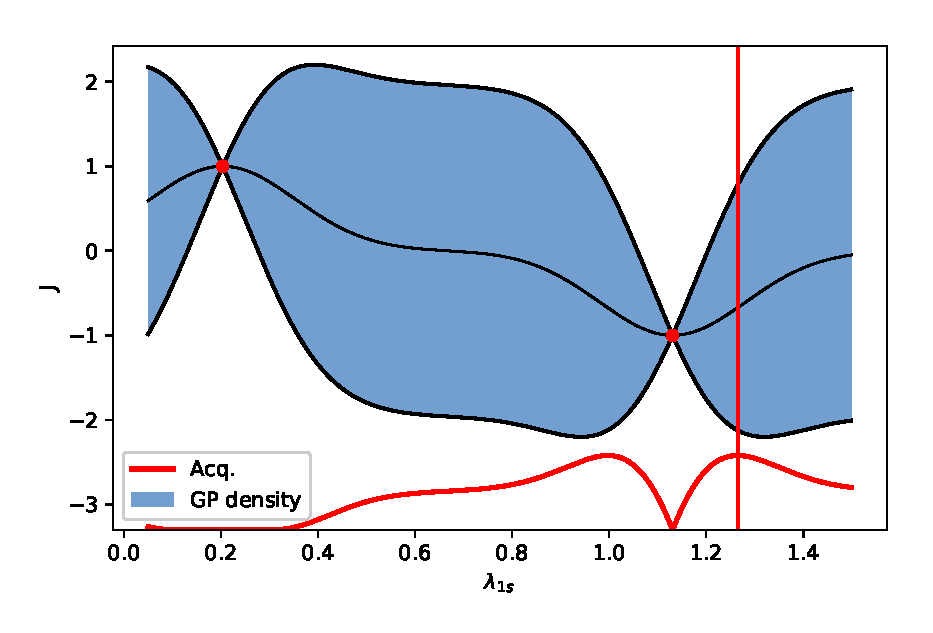
\includegraphics[width=0.9\textwidth]{figures/gp/lam1s_init2.eps}};
  \node<2> (max1) {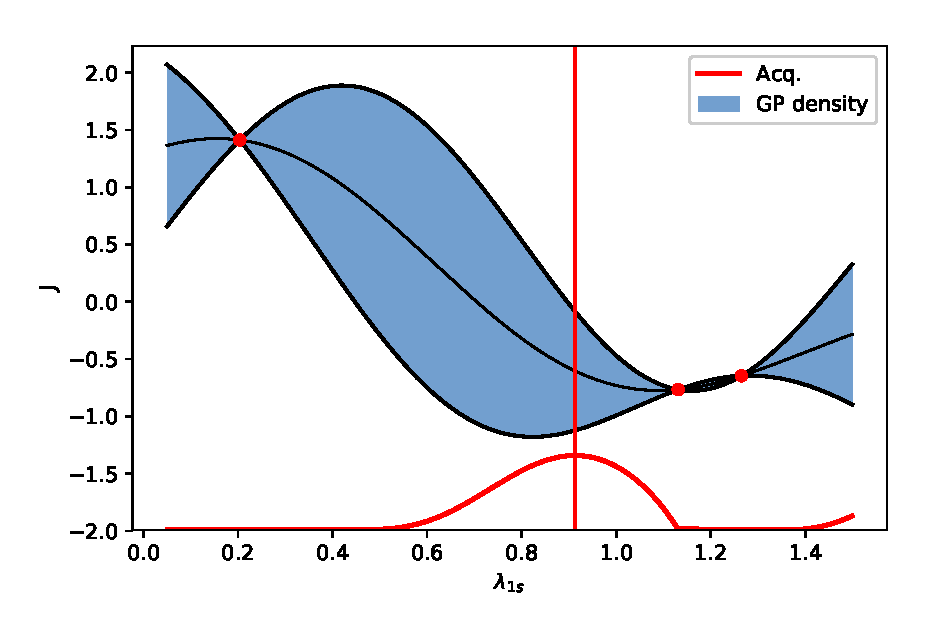
\includegraphics[width=0.9\textwidth]{figures/gp/lam1s_init2_maxevals1.eps}};
  \node<3> (max2) {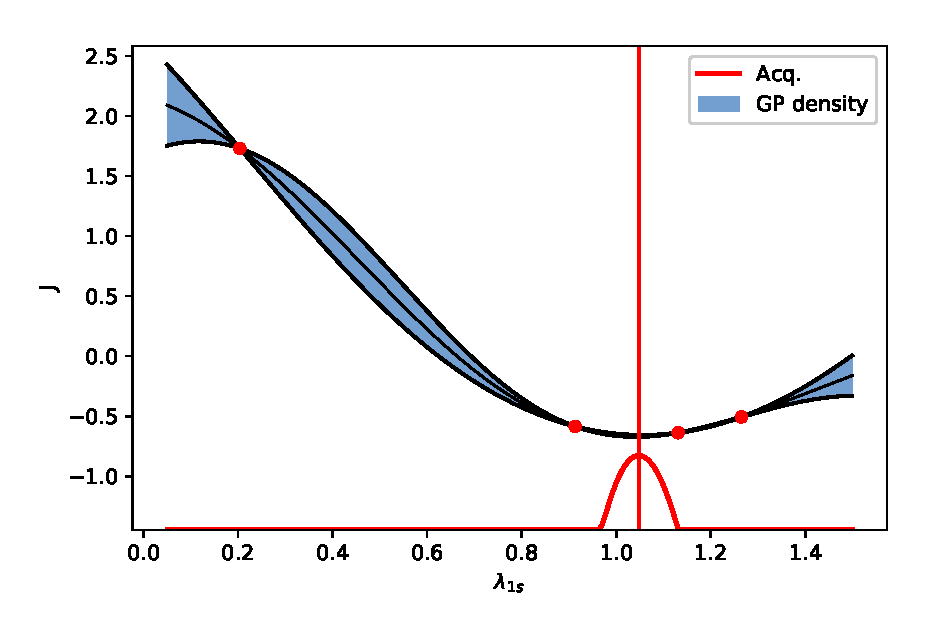
\includegraphics[width=0.9\textwidth]{figures/gp/lam1s_init2_maxevals2.eps}};
  \node<4> (max3) {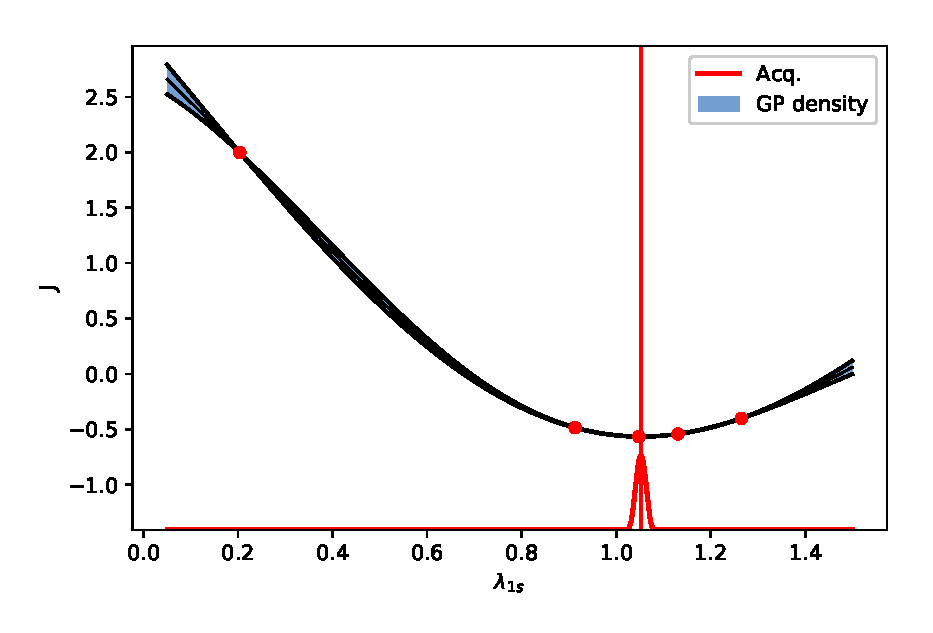
\includegraphics[width=0.9\textwidth]{figures/gp/lam1s_init2_maxevals3.eps}};
\end{tikzpicture}
\end{frame}
%%%%%%%%%%%%%%%%%%%%%%%%%%%%%%%%%%%%%%%%%%%%%%%%%%%%%%%%%%%%%%%%%%%%%%%%
\end{document}
